\documentclass{beamer}
%\usetheme{Boadilla}
\usetheme{DarkConsole}
\usepackage[backend=biber]{biblatex}
\addbibresource{ref.bib}
\usepackage{courier}
\usepackage[T1]{fontenc}
\usepackage{multicol}
\usepackage{tikz}
\usetikzlibrary{calc}
\usepackage{hyperref}
\hypersetup{
    colorlinks=true,
    linkcolor=whiteee,
    filecolor=gold,
    urlcolor=gold,
	citecolor=gold,
    pdftitle={Overleaf Example},
    pdfpagemode=FullScreen,
    }
\usepackage{graphicx}
\usepackage{chronology}

\definecolor{lightgreen}{RGB}{127,255,0} \definecolor{myblack}{RGB}{68,68,68}
\definecolor{mygreen}{RGB}{64,128,0}
\setbeamercolor{block title}{bg=mygreen,fg=white}
\setbeamercolor{block body}{bg=myblack,fg=white}

\graphicspath{ {./assets} }

\title {AWS}
\author {Henrique Tsuyoshi Yara}
\institute {OPUS-software}

\begin{document}

\begin{frame}{\titlepage}
	\begin{figure}[htpb]
		\centering
		\includegraphics[width=0.5\textwidth]{aws-logo}
		\caption{AWS logo}
	\end{figure}
\end{frame}

\begin{frame}{Índice}
\begin{multicols}{2}
  \tableofcontents
\end{multicols}
\end{frame}

%\setbeamercovered{transparent}

\section{História}

\begin{frame}
	\frametitle{Curiosidade}
	\begin{figure}[htpb]
		\centering
		\includegraphics[width=0.6\textwidth]{server_cluster}
		\caption{A cluster of servers drawn in a system diagram \footnote{\href{https://www.youtube.com/watch?v=e3UMvBP2RRo}{Image source link}}}
	\end{figure}
\end{frame}

\subsection{Linha do tempo}

\begin{frame}
	\frametitle{Linha do tempo}
	\begin{center}
		História da computação em nuvem\cite{CCHistory}
	\end{center}
	\hfill
	\begin{scriptsize}
	\begin{bf}
	\begin{center}
		\begin{chronology}[10]{1955}{2010}{12cm}[\textwidth]
			\event[1955]{1965}{1955-1965}
			\event[1970]{1990}{1970-1990}
			\event[1990]{2006}{1990-2006}
			\event{2006}{2006}
			\event[2006]{2010}{2016-2010}
		\end{chronology}
	\end{center}
	\end{bf}
	\hfill
	\begin{itemize}
		\item (1955-1965) Problemas na infraestrutura de TI
		\item (1970-1990) Hypervisors e a internet
		\item (1990-2006) Internet para todos
		\item (2006-2006) Precipitation
		\item (2006-2010) Primeiros dias da computação em nuvem
	\end{itemize}
	\end{scriptsize}
\end{frame}

\begin{frame}
	\frametitle{Linha do tempo}
	\begin{center}
		Problemas na infraestrutura de TI \\ (1955-1965)
	\end{center}
	\hfill
	\begin{scriptsize}
	\begin{bf}
	\begin{center}
		\begin{chronology}[10]{1955}{2010}{12cm}[\textwidth]
			\color{lightgreen}
				\event[1955]{1965}{1955-1965}
		\end{chronology}
	\end{center}
	\end{bf}
	\end{scriptsize}
\end{frame}

\begin{frame}[allowframebreaks]
	\frametitle{Problemas na infraestrutura de TI}
	\begin{itemize}
		\item 1942 - John Vincent Atanasoff construiu o computador ABC
		\item 1960 - Muito caro para aderir os computadores
			\begin{itemize}
				\item Sala inteira para o servidor (Manter temperatura ideal, espaço, etc\dots)
				\item Computador
				\item Funcionários especializados
				\item Problemas para adaptar o software
			\end{itemize}
		\framebreak
		\item Empresas com poder aquisitivo conseguiram aderir os computadores
		\item 1961 - John MacCharty fez uma palestra no MIT
			\begin{itemize}
				\item Computação poderia ser vendida como água ou eletricidade \cite{SimsonTCI}
				\item Mas seria necessário de uma grande evolução tecnológica
			\end{itemize}
	\end{itemize}
\end{frame}

\begin{frame}
	\frametitle{Linha do tempo}
	\begin{center}
		Hypervisors e a internet \\
		(1970-1990)
	\end{center}
	\hfill
	\begin{scriptsize}
	\begin{bf}
	\begin{center}
		\begin{chronology}[10]{1955}{2010}{12cm}[\textwidth]
			\color{lightgreen}
				\event[1970]{1990}{1970-1990}
		\end{chronology}
	\end{center}
	\end{bf}
	\end{scriptsize}
\end{frame}

\begin{frame}[allowframebreaks]
	\frametitle{Hypervisors e a internet}
	\begin{itemize}
		\item Diminiur os custos da adoção do computador
			\begin{itemize}
				\item Múltiplos usuários podem compartilhar o mesmo armazenamento e o poder de processamento da CPU
			\end{itemize}
		\item 1970 - Nasceu a tecnologia da virtualização
			\begin{itemize}
				\item Um host pode ser particionado em VMs
				\item Cada parte pode rodar um código independente
			\end{itemize}
		\framebreak
		\item 1983 - A internet nasceu
			\begin{itemize}
				\item Projeto ARPANet: comunicação de professores de universidades
			\end{itemize}
		\item Arquitetura cliente-servidor conectados por cabos (Internet)
		\item O número de servers cresceram junto com as páginas web
			\begin{itemize}
				\item Os servers se moveram para datacenters
			\end{itemize}
	\end{itemize}
\end{frame}

\begin{frame}
	\frametitle{Linha do tempo}
	\begin{center}
		Internet para todos \\
		(1990-2006)
	\end{center}
	\hfill
	\begin{scriptsize}
	\begin{bf}
	\begin{center}
		\begin{chronology}[10]{1955}{2010}{12cm}[\textwidth]
			\color{lightgreen}
				\event[1990]{2006}{1990-2006}
		\end{chronology}
	\end{center}
	\end{bf}
	\end{scriptsize}
\end{frame}

\begin{frame}
	\frametitle{Internet para todos}
	\begin{itemize}
		\item Empresas precisavam de datacenters maiores
		\item Problemas:
			\begin{itemize}
				\item Ociosidade dos servers (off-season)
				\item Escalabilidade manual e precisava de dispositivos físicos
					\begin{itemize}
						\item Difícil acompanhar o crescimento da aplicação
					\end{itemize}
				\item Atualização e manutenção manuais
				\item Grande distância dos servidores (UX ruim)
			\end{itemize}
	\end{itemize}
\end{frame}

\begin{frame}
	\frametitle{Linha do tempo}
	\begin{center}
		Precipitation \\
		(2006)
	\end{center}
	\hfill
	\begin{scriptsize}
	\begin{bf}
	\begin{center}
		\begin{chronology}[10]{1955}{2010}{12cm}[\textwidth]
			\color{lightgreen}
				\event{2006}{2006}
		\end{chronology}
	\end{center}
	\end{bf}
	\end{scriptsize}
\end{frame}

\begin{frame}[allowframebreaks]
	\frametitle{Precipitação}
	\begin{itemize}
		\item Grandes players (\it{Google, Amazon, eBay, etc\dots})
			\begin{itemize}
				\item Próprio \it{data center}
				\item Centenas/milhares de servers de alta qualidade no mundo inteiro
				\item Começar a alugar essas máquinas
			\end{itemize}
		\item 2006 - "Cloud Computing" introduzino como forma de aluguel de poder computacional
		\item AWS - primeira provedora de cloud
		\item Sonho de John McCharty foi realizado depois de 50 anos
	\end{itemize}
\end{frame}

\begin{frame}
	\frametitle{Linha do tempo}
	\begin{center}
		Primeiros dias da computação em nuvem \\
		(2006-2010)
	\end{center}
	\hfill
	\begin{scriptsize}
	\begin{bf}
	\begin{center}
		\begin{chronology}[10]{1955}{2010}{12cm}[\textwidth]
			\color{lightgreen}
				\event[2006]{2010}{2016-2010}
		\end{chronology}
	\end{center}
	\end{bf}
	\end{scriptsize}
\end{frame}

\begin{frame}[allowframebreaks]
	\frametitle{Primeiros dias da computação em nuvem}
	\begin{itemize}
		\item Por 6 anos a AWS estabeleceu seu monopólio na área de nuvem
		\item Computação em nuvem $\rightarrow$ empresa focam no desenvolvimento
			\begin{itemize}
				\item Os dados são criptografados e seguros
				\item Dados são armazenados com redundância em nuvem
				\item Escalabilidade
				\item De fácil deploy
				\item Alta disponibilidade
			\end{itemize}
	\end{itemize}
\end{frame}

\section{Conceito}

\subsection{Cloud X Virtualização}

\begin{frame}
	\frametitle{Virtualização}
	\begin{itemize}
		\item Criação de infraestruturas virtuais a partir de uma estrutura física
	\end{itemize}
\end{frame}

\begin{frame}
	\frametitle{Cloud}
	\begin{itemize}
		\item Conceito que reúne vários \textit{softwares} e utiliza de virtualização
		\item Possui algumas características específicas:
			\begin{itemize}
				\item Autoserviço sob demanda
				\item Amplo acesso a rede
				\item Pool de recursos
				\item Rápida elaticidade
				\item Serviços mensuráveis
			\end{itemize}
		\item \textbf{Colocation}: alugar determinado espaço de um Data Center (refrigeração, instalação elétrica e segurança). No entanto, utiliza seu próprio equipamento. \footnote{\href{https://vivomeunegocio.com.br/conteudos-gerais/expandir/cloud-colocation-data-center}{Colocation}}
	\end{itemize}
\end{frame}

\subsection{NIST}

\begin{frame}
	\frametitle{O que é cloud para o NIST}
	\begin{itemize}
		\item Um modelo para habilitar o acesso por rede a um conjunto compartilhado de \textbf{recursos de computação} e precisa ser:
			\begin{itemize}
				\item Ubíquo (Pode ser encontrado em todos os lugares)
				\item Conveniente
				\item Sob demanda
			\end{itemize}
		\item \textbf{Recursos de computação}: Redes, servidores, armazenamento, aplicações e serviços
		\item Esses recursos devem ser provisionados e liberados com o mínimo de esforço de gerenciamento ou interação com o provedor de serviços.
	\end{itemize}
\end{frame}

\begin{frame}
	\frametitle{5 Características}
	\begin{itemize}
		\item Conceito que reúne vários \textit{softwares} e utiliza de virtualização
		\item Possui algumas características específicas (NIST):
			\begin{itemize}
				\item Autoserviço sob demanda
				\item Amplo acesso a rede
				\item Pool de recursos
				\item Rápida elaticidade
				\item Serviços mensuráveis
			\end{itemize}
	\end{itemize}
\end{frame}

\begin{frame}
	\frametitle{Auto-serviço sob demanda}
	\begin{itemize}
		\item O consumidor pode providionar por conta própra \textbf{Recursos de computação}
		\item Não necessita da intervenção humana dos provedores de serviço
	\end{itemize}
\end{frame}

\begin{frame}
	\frametitle{Amplo acesso por rede}
	\begin{itemize}
		\item Os \textbf{Recursos de computação} estão disponíveis através da rede
		\item São acessados através de mecanismos padronizados que promovem o uso por dispositivos, clientes leves ou ricos de diversas plataformas (Smartphones, tablets, laptops ou desktops)
	\end{itemize}
\end{frame}

\begin{frame}
	\frametitle{Agrupamento de recursos}
	\begin{itemize}
		\item Os \textbf{Recusos de computação} do provedor são agrupados para atender a múltiplos consumidores em modalidade multi-inquilinos (Recursos físicos e virtuais diferentes dinamicamentes atribuídos e reatribuídos conforme a demanda dos consumidores)
		\item Há uma certa independência de localização geográfica, uma vez que o consumidor em geral não controla ou conhece a localização exata dos recursos fornecidos
		\item Mas pode ser capaz de especificar a localização em um nível de abstração mais alto (país, estado, datacenter)
	\end{itemize}
\end{frame}

\begin{frame}
	\frametitle{Elasticidade rápida}
	\begin{itemize}
		\item Os recursos podem ser provisionados e liberados elasticamente, em alguns casos automaticamentes, para rapidamente aumentar ou diminuir de acordo com a demanda
		\item Para o consumidor, os recursos disponíveis para provisionamento muitas vezes parecem ser ilimitados e podem ser alocados em qualquer quantidade e a qualquer tempo
	\end{itemize}
\end{frame}

\begin{frame}
	\frametitle{Serviços mensurado}
	\begin{itemize}
		\item Os sistemas na nuvem automaticamente controlam e otimizam o uso dos recursos através de medições em um nível de abstração apropriado para o tipo de serviço (como armazenamento, processamento, comunicação de ree e contas de usuário ativas)
		\item A utilização de recursos pode ser monitorada, controlada e informada, gerando transparência tanto para o fornecedor como para o consumidor do serviço utilizado
	\end{itemize}
\end{frame}

\begin{frame}
	\frametitle{Primeiros dias da computação em nuvem}
	\begin{figure}[htpb]
	\begin{center}
	\begin{tiny}
	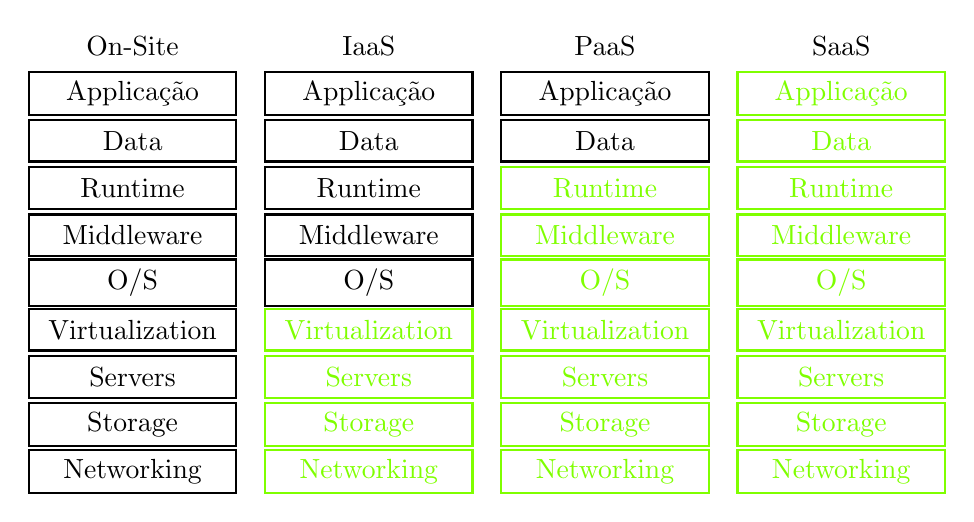
\begin{tikzpicture}[scale=1, transform shape]
		\node (A) at (0,4) {\normalsize On-Site};
		\node (A1) at ($(A) - (0,0.6)$)  [draw,thick,minimum width=75,minimum height=15] {Applicação};
		\node (A2) at ($(A1) - (0,0.6)$) [draw,thick,minimum width=75,minimum height=15] {Data};
		\node (A3) at ($(A2) - (0,0.6)$) [draw,thick,minimum width=75,minimum height=15] {Runtime};
		\node (A4) at ($(A3) - (0,0.6)$) [draw,thick,minimum width=75,minimum height=15] {Middleware};
		\node (A5) at ($(A4) - (0,0.6)$) [draw,thick,minimum width=75,minimum height=15] {O/S};
		\node (A6) at ($(A5) - (0,0.6)$) [draw,thick,minimum width=75,minimum height=15] {Virtualization};
		\node (A7) at ($(A6) - (0,0.6)$) [draw,thick,minimum width=75,minimum height=15] {Servers};
		\node (A8) at ($(A7) - (0,0.6)$) [draw,thick,minimum width=75,minimum height=15] {Storage};
		\node (A9) at ($(A8) - (0,0.6)$) [draw,thick,minimum width=75,minimum height=15] {Networking};
		\node (B) at (3,4) {\normalsize IaaS};
		\node (B1) at ($(B) - (0,0.6)$)  [draw,thick,minimum width=75,minimum height=15] {Applicação};
		\node (B2) at ($(B1) - (0,0.6)$) [draw,thick,minimum width=75,minimum height=15] {Data};
		\node (B3) at ($(B2) - (0,0.6)$) [draw,thick,minimum width=75,minimum height=15] {Runtime};
		\node (B4) at ($(B3) - (0,0.6)$) [draw,thick,minimum width=75,minimum height=15] {Middleware};
		\node (B5) at ($(B4) - (0,0.6)$) [draw,thick,minimum width=75,minimum height=15] {O/S};
		\node (B6) at ($(B5) - (0,0.6)$) [lightgreen,draw,thick,minimum width=75,minimum height=15] {Virtualization};
		\node (B7) at ($(B6) - (0,0.6)$) [lightgreen,draw,thick,minimum width=75,minimum height=15] {Servers};
		\node (B8) at ($(B7) - (0,0.6)$) [lightgreen,draw,thick,minimum width=75,minimum height=15] {Storage};
		\node (B9) at ($(B8) - (0,0.6)$) [lightgreen,draw,thick,minimum width=75,minimum height=15] {Networking};
		\node (C) at (6,4) {\normalsize PaaS};
		\node (C1) at ($(C) - (0,0.6)$)  [draw,thick,minimum width=75,minimum height=15] {Applicação};
		\node (C2) at ($(C1) - (0,0.6)$) [draw,thick,minimum width=75,minimum height=15] {Data};
		\node (C3) at ($(C2) - (0,0.6)$) [lightgreen,draw,thick,minimum width=75,minimum height=15] {Runtime};
		\node (C4) at ($(C3) - (0,0.6)$) [lightgreen,draw,thick,minimum width=75,minimum height=15] {Middleware};
		\node (C5) at ($(C4) - (0,0.6)$) [lightgreen,draw,thick,minimum width=75,minimum height=15] {O/S};
		\node (C6) at ($(C5) - (0,0.6)$) [lightgreen,draw,thick,minimum width=75,minimum height=15] {Virtualization};
		\node (C7) at ($(C6) - (0,0.6)$) [lightgreen,draw,thick,minimum width=75,minimum height=15] {Servers};
		\node (C8) at ($(C7) - (0,0.6)$) [lightgreen,draw,thick,minimum width=75,minimum height=15] {Storage};
		\node (C9) at ($(C8) - (0,0.6)$) [lightgreen,draw,thick,minimum width=75,minimum height=15] {Networking};
		\node (D) at (9,4) {\normalsize SaaS};
		\node (D1) at ($(D) - (0,0.6)$)  [lightgreen,draw,thick,minimum width=75,minimum height=15] {Applicação};
		\node (D2) at ($(D1) - (0,0.6)$) [lightgreen,draw,thick,minimum width=75,minimum height=15] {Data};
		\node (D3) at ($(D2) - (0,0.6)$) [lightgreen,draw,thick,minimum width=75,minimum height=15] {Runtime};
		\node (D4) at ($(D3) - (0,0.6)$) [lightgreen,draw,thick,minimum width=75,minimum height=15] {Middleware};
		\node (D5) at ($(D4) - (0,0.6)$) [lightgreen,draw,thick,minimum width=75,minimum height=15] {O/S};
		\node (D6) at ($(D5) - (0,0.6)$) [lightgreen,draw,thick,minimum width=75,minimum height=15] {Virtualization};
		\node (D7) at ($(D6) - (0,0.6)$) [lightgreen,draw,thick,minimum width=75,minimum height=15] {Servers};
		\node (D8) at ($(D7) - (0,0.6)$) [lightgreen,draw,thick,minimum width=75,minimum height=15] {Storage};
		\node (D9) at ($(D8) - (0,0.6)$) [lightgreen,draw,thick,minimum width=75,minimum height=15] {Networking};
	\end{tikzpicture}
	\end{tiny}
	\end{center}
	\caption{Imagem retirado do site da redhat\footnote{\href{https://www.redhat.com/cms/managed-files/iaas-paas-saas-diagram5.1-1638x1046.png}{RedHat IaaS, PaaS e SaaS}}}
	\end{figure}
\end{frame}

\subsection{Tipos de nuvem}

\begin{frame}
	\frametitle{Tipos de nuvem}
	\begin{itemize}
		\item \textbf{Infraestrutura como Serviço (Iaas)}
		\item \textbf{Software como Serviço (SaaS)}
		\item \textbf{Plataforma como Serviço (PaaS)}
	\end{itemize}
\end{frame}

\begin{frame}
	\frametitle{IaaS - Infrastructure as a Service}
	\begin{itemize}
		\item O recurso fornecido ao consumidor é provisionar:
			\begin{itemize}
				\item Processamento
				\item Armazenamento
				\item Comunicação de rede
				\item Outros recursos de computação funcamentais nos quais o consumidor pode instalar e executar softwares em geral, incluindo sistemas operaionais e aplicativos
				\item Possivelmente um controle limitado de alguns componentes de rede (\textit{firewall})
			\end{itemize}
	\end{itemize}
\end{frame}

\begin{frame}
	\frametitle{PaaS - Plataform as a Service}
	\begin{itemize}
		\item O recurso fornecido ao consumidor é instalar na infraestrutura na nuvem aplicativos criados ou adiquiridos pelo consumidor
		\item O consumidor tem controle sobre as aplicações instaladas e possívelmente configuraçoes de hospedagem de aplicações
		\item O consumidor não gerencia nem controla a infraestrutura na nuvem subjacente (Rede, servidores, sistemas operacionais, armazenamento ou mesmo recursos individuais da aplicação, com a possível exeção de configurações limitadas por usuário)
	\end{itemize}
\end{frame}

\begin{frame}
	\frametitle{SaaS - Software as a Service}
	\begin{itemize}
		\item O recurso fornecido ao consumidor é o uso de aplicções do fornecedor executando em uma infraestrutura na nuvem
		\item As aplicações podem ser acessadas por vários dispositivos clientes através de interfaces leves ou ricas
		\item O consumidor não gerencia nem controla a infraestrutura na nuvem subjacente (Rede, servidores, sistemas operacionais, armazenamento ou mesmo recursos individuais da aplicação, com a possível exeção de configurações limitadas por usuário)
	\end{itemize}
\end{frame}

\begin{frame}
	\frametitle{Exemplos}
	\begin{tiny}
	\begin{table}[ht]
		\centering
		\begin{tabular}{|p{1cm}|p{5cm}|p{4cm}|}
		\hline
			Tipo & Serviço & Exemplos \\
		\hline
		\hline
		  \multirow{3}{*}{IaaS}
			& Rede virtualizada & AWS VPC, Azura Virtual Network \\
			& Armazenamento de dados & AWS S3, Google cloud storage \\
			& Servidores Virtuais & AWS EC2, Azure Virtual Machines \\
			\hline
		  \multirow{2}{*}{PaaS}
			& Infraestrutura para desenvolvimento, implantação e execução de aplicativos & Heroku, Google App Engine \\
			& Plataforma testes e gerenciamento de aplicações & AWS Elastic Beanstalk \\
			\hline
		  \multirow{3}{*}{SaaS}
			& Armazenamento Dados & DropBox, Google Drive \\
			& Editor de textos e planilha & Gsuite e Office 365 \\
			& SIstema de Gestão de banco de dados & AWS RDS, Google Cloud SQL \\
		\hline
		\end{tabular}
		\caption{Exemplos de serviços}
	\end{table}
	\end{tiny}
\end{frame}

\subsection{Modelos de implementação de nuvem}

\begin{frame}
	\frametitle{Modelos de implementação de nuvem}
	\begin{itemize}
		\item Nuvem pública
		\item Nuvem privada
		\item Nuvem híbrida
		\item Nuvem comunitária
	\end{itemize}
\end{frame}

\begin{frame}
	\frametitle{Nuvem pública}
	\begin{itemize}
		\item Provisionada para uso aberto ao público em geral
		\item Sua propriedade, gerenciamento e operação podem ser de:
			\begin{itemize}
				\item Uma empresa
				\item Uma instituição acadêmica
				\item Uma organização do governo
				\item Ou uma combinação mista
			\end{itemize}
		\item Fica nas instalações do fornecedor
	\item \textbf{OBS}: Criar uma estrutura na Amazon e configurar usando VPN ou conexão direta continua sendo uma nuvem pública
	\end{itemize}
\end{frame}

\begin{frame}
	\frametitle{Nuvem privada}
	\begin{itemize}
		\item Provisionada para uso exclusivo por uma únic organização composta de diversos consumidores
		\item A sua propriedade, gerenciamento de operação podem ser de:
			\begin{itemize}
				\item A própria organização
				\item Terceiros
				\item Combinação mista
			\end{itemize}
		\item Pode estar dentro ou fora das instalações da organização
		\item Nuvem privada não é organização e não precisa estar instalada localmente
	\end{itemize}
\end{frame}

\begin{frame}
	\frametitle{Nuvem comunitária}
	\begin{itemize}
		\item Provisionada para uso exclusivo por uma determinada comunidade de consumidores de organizações que têm interesses em comum (missão, requisitos de segurança, políticas, observância de regulamentações)
		\item A sua propriedade, gerenciamento e operação podem ser de:
			\begin{itemize}
				\item Uma organização
				\item Mais de uma organizações da comunidade
				\item Terceiros
				\item Combinação mista
			\end{itemize}
		\item Pode estar dentro ou fora das instalações das organizações participantes
	\end{itemize}
\end{frame}

\begin{frame}
	\frametitle{Nuvem híbrida}
	\begin{itemize}
		\item Composição de duas ou mais infraestruturas na nuvem (\textbf{privadas}, \textbf{comunitárias} ou \textbf{públicas}) que permanecem entidades distintas
		\item São interligadas por tecnoogia padronizada ou proprietária que permite a comunicação de dados e portabilidade de aplicações (Transferencia de processamento para a nuvem para balanceamento de carga entre nuvens)
	\end{itemize}
\end{frame}


\include{./chapters/CloudVs.tex}
\section{AWS}

\subsection{Origem}

\begin{frame}[allowframebreaks]
	\frametitle{Origem AWS}
	\begin{itemize}
		\item 2006 - Amazon Web Services começou a oferecer infraestrutura de TI como forma de serviços web
			\begin{itemize}
				\item Low Cost (Pay-as-you-go)
				\item Agility and Instant Elasticity
				\item Open and Flexible
				\item Secure (PCI DSS Level 1, ISO27001, etc\dots)
			\end{itemize}
			\framebreak
		\item Instância (2006):
			\begin{itemize}
				\item 1.7 GHz Xeon Processor
				\item 1.75 GB of RAM
				\item 160 GB of local disk
				\item 250 Mbps network bandwidth
			\end{itemize}
		\item Instância (2019):
			\begin{itemize}
				\item 4.0 GHz Xeon Processor (z1d instance)
				\item 24 TiB of RAM (High Memory instances)
				\item 60 TB of NVMe local storage (I3en.metal instances)
				\item 100 Gbps network bandwidth
			\end{itemize}
	\end{itemize}
\end{frame}

\subsection{Formas de acesso}

\begin{frame}
	\frametitle{Formas de acesso}
	\begin{itemize}
		\item \textbf{Console}: Gerenciar a infraestrutura e os recursos da aws com uma interface web
		\item \textbf{SDK}: Simplifica o uso dos serviços da AWS provendo bibliotecas para os desenvolvedores
			\begin{itemize}
				\item Tem suporte para: Java, .NET, C++, PHP, etc\dots
			\end{itemize}
		\item \textbf{CLI}: Controla múltiplos serviços usando a linha de comando e é possível automatizar usando scripts
	\end{itemize}
\end{frame}

\section{Introdução}

\begin{frame}
	\frametitle{Recursos}
	\begin{itemize}
		\item Cada recurso vai ter um \textbf{Amazon Resource name} (Identificador único)
		\item Free Tier
			\begin{itemize}
				\item São recursos que podem ser usadas de graça na Amazon
			\end{itemize}
		\item Calculadora
			\begin{itemize}
				\item \href{https://calculator.s3.amazonaws.com/index.html}{Calculadora antiga}
				\item \href{https://calculator.aws/}{Calculadora nova}
			\end{itemize}
	\end{itemize}
\end{frame}

\begin{frame}
	\frametitle{Regiões}
	\begin{itemize}
		\item Cada região tem um preço diferente
		\item Uma região é composta de zonas de disponibilidade
		\item Algumas regiões podem ter mais serviços que outras
		\item \textbf{OBS}: É bom saber se juridicamente a gente pode armazenar os dados fora do Brasil
			\begin{itemize}
				\item \href{https://aws.amazon.com/pt/about-aws/global-infrastructure/regions_az/}{Regiões e zonas de disponibilidade}
				\item \href{https://aws.amazon.com/pt/about-aws/global-infrastructure/regional-product-services/}{Serviços regionais}
			\end{itemize}
		\item \textbf{OBS}: Tráfegos entre zonas de disponibilidade ou regiões podem acabar sendo cobrados
	\end{itemize}
\end{frame}

\begin{frame}
	\frametitle{Zonas de disponibilidade}
	\begin{itemize}
		\item Compõem as regiões
		\item Para verificar o status das zonas de disponibilidade/regiões ou recursos
			\begin{itemize}
				\item \href{http://status.aws.amazon.com/}{Status AWS}
			\end{itemize}
	\frametitle{Pontos de presença}
	\begin{itemize}
		\item Pontos de cache utilizado pela AWS (É possível usar \textit{CNDs})
	\end{itemize}
	\end{itemize}
\end{frame}


\section{Virtual Private Cloud}

\begin{frame}
	\frametitle{Virtual Private Cloud (VPC)}
	\begin{itemize}
		\item VPCs são isoladas entre si, mas podem ser configuradas para se comunicarem
		\item Cada região tem uma VPC padrão, mas é recomendada criar sua própria VPC para o ambiente de produção
		\item Dentro de uma VPC é possível criar uma subnet
		\item As subnets são aplicadas em AZs (Zonas de disponibilidade)
		\item Subnet:
			\begin{itemize}
				\item Pública: Pode ser acessada remotamente por qualquer lugar
				\item Privada: Só vai ser acessível por dentro da AWS
			\end{itemize}
		\item \textbf{VPC wizard} tem algumas configurações pré-definidas de VPC
		\item Lembrar de verificar e configurar:
		\begin{itemize}
			\item DHCP options set
			\item DNS resolution
			\item DNS hostname
		\end{itemize}
	\end{itemize}
\end{frame}

\begin{frame}
	\frametitle{NAT Gateway}
	\begin{itemize}
		\item Instâncias dentro de subnets privadas podem conectar com serviços fora da VPC, mas instâncias de fora não podem iniciar ocnexões com essas instâncias
			\begin{itemize}
				\item Public: Instâncias em subnets privadas podem conectar com a internet
				\item Private: Instâncias em subnets privadas podem conectar com outros VPCs
			\end{itemize}
		\item Cobrança por hora de uso e quantidade em GBs de dados processados
	\end{itemize}
\end{frame}

\begin{frame}
	\frametitle{Internet Gateway}
	\begin{itemize}
		\item Permite a comunicação do seu VPC com a internet
		\item Libera a entrada e a saída de determinado \textbf{Route Table}
		\item Não tem custo
	\end{itemize}
\end{frame}

\begin{frame}
	\frametitle{Route table}
	\begin{itemize}
		\item Associa as \textbf{subnets}
		\item Se a \textbf{Route table} não tiver uma rota default ela não está pública
	\end{itemize}
\end{frame}

\begin{frame}
	\frametitle{Security Groups X NetworkACL}
	\begin{itemize}
		\item \textbf{Securty Groups}
		\begin{itemize}
			\item Opera no nível de instância (Primeira camada de defesa)
			\item Apenas regras de liberação
			\item Stateful: o tráfego de retorno é automaticamente permitido, independentemente de quaisquer regras
			\item Aplica-se a uma instância somente quando especificado o grupo de segurança
		\end{itemize}
		\item \textbf{NetworkACL}
		\begin{itemize}
			\item Regra de segurança da rede (Como se fosse um \textit{firewall})
			\item Regras de liberação e negação
			\item Stateless: o tráfego de retorno deve ser explicitamente permitido pelas regras
			\item Aplica a todas as instâncias nas sub-redes
		\end{itemize}
	\end{itemize}
\end{frame}

\begin{frame}
	\frametitle{NetworkACL}
	\begin{itemize}
		\item Cada regra vai ter uma prioridade
		\item É bom deixar um espaço entre cada regra para possíveis regras futuras (Ex: deixar 10 espaços entre cada regra)
		\item \textbf{OBS}: É bom liberar portas efêmeras (1024-65535). São usadas para comunicações de saída através do protocolo de rede TCP/IP
	\end{itemize}
\end{frame}

\begin{frame}
	\frametitle{Network Optimization}
	\begin{itemize}
		\item Quantas VPCs eu preciso?
			\begin{itemize}
				\item Depende de quanto achar necessário para separar a aplicação
				\item É comum uma VPC Para AWS Network Firewall ou Firewall com Gateway Load Balancer.
				\item Talvez VPCs para Ingress e Egress centralizados
			\end{itemize}
		\item Tamanho da VPC
			\begin{itemize}
				\item Evitar alocar /16 endereços IP padrão para todas as VPCs
				\item Alguns recursos precisam de IPs livres (Load balancer precisa de 8 IPs livres)
				\item É possível usar o IPAM (VPC IP Address Manager)\footnote{\href{Network Address Management and Auditing at Scale with Amazon VPC IP Address Manager}{https://aws.amazon.com/blogs/aws/network-address-management-and-auditing-at-scale-with-amazon-vpc-ip-address-manager/}} para gerenciar os IPs nas redes
				\item OBS: É possível usar o cloudWatch junto com o IPAM para verificar se os endereços IPs estão acabando
			\end{itemize}
		\item Quantas subnets por VPC?
			\begin{itemize}
				\item Pelo menos 1 subnet por VPC
				\item Caso a aplicação esteja em várias AZs, é recomendado pelo menos uma subnet por AZ
				\item OBS: Quando uma subnet é colocada em uma AZ não é possível mudar
			\end{itemize}
		\item Comparilhar VPC ou criar uma VPC nova para o workload?
			\begin{itemize}
				\item Mesmo que diferentes times trabalhem em diferentes contas da AWS, não significa que precisam necessariamente usar diferentes VPCs
				\item VPC Sharing\footnote{\href{VPC Sharing}{https://aws.amazon.com/blogs/networking-and-content-delivery/vpc-sharing-a-new-approach-to-multiple-accounts-and-vpc-management/}} permite compartilhar VPCs com outras contas AWS
				\item \href{VPC Sharing Best Pratices}{https://aws.amazon.com/blogs/networking-and-content-delivery/vpc-sharing-key-considerations-and-best-practices/}
			\end{itemize}
	\end{itemize}
\end{frame}


\section{EC2}

\begin{frame}
	\frametitle{EC2}
	\begin{itemize}
		\item Oferece instâncias onde podemos escolher: Processador, Sistema Operacional, Armazenamento, Rede
		\begin{figure}[htpb]
		\begin{center}
		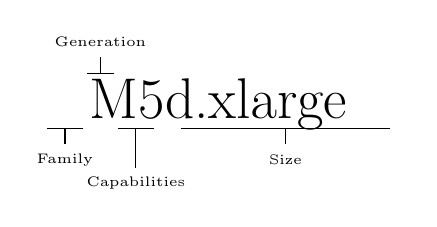
\begin{tikzpicture}[scale=1, transform shape]
			\node at (0,0) {\huge M5d.xlarge};
			\node (M1) at (-2.3,-0.3) {};
			\node (M2) at (-1.6,-0.3) {};

			\draw (M1)--(M2);
			\draw ($(M1)!0.5!(M2)$)--($(M1)!0.5!(M2) - (0,0.2)$);
			\node at ($(M1)!0.5!(M2) - (0,0.4)$) {\tiny Family};

			\node (C1) at (-1.8,0.4) {};
			\node (C2) at (-1.2,0.4) {};

			\draw (C1)--(C2);
			\draw ($(C1)!0.5!(C2)$)--($(C1)!0.5!(C2) + (0,0.2)$);
			\node at ($(C1)!0.5!(C2) + (0,0.4)$) {\tiny Generation};

			\node (D1) at (-1.4,-0.3) {};
			\node (D2) at (-0.7,-0.3) {};

			\draw (D1)--(D2);
			\draw ($(D1)!0.5!(D2)$)--($(D1)!0.5!(D2) - (0,0.5)$);
			\node at ($(D1)!0.5!(D2) - (0,0.7)$) {\tiny Capabilities};

			\node (T1) at (-0.6,-0.3) {};
			\node (T2) at (2.3,-0.3) {};

			\draw (T1)--(T2);
			\draw ($(T1)!0.5!(T2)$)--($(T1)!0.5!(T2) - (0,0.2)$);
			\node at ($(T1)!0.5!(T2) - (0,0.4)$) {\tiny Size};
		\end{tikzpicture}
		\end{center}
		\caption{Tipo das instâncias}
		\label{fig:}
		\end{figure}
 		\item São para propósito geral, podem ser usadas em: Web/App servers, Enterprise apps, Gaming servers, caching Fleets, Analytics applications, Dev/Test Environments, etc\dots
	\end{itemize}
\end{frame}

\subsection{Tipo de instâncias}

\begin{frame}
	\frametitle{Instâncias de propósito geral}
	\begin{itemize}
		\item \textbf{Instâncias M5}: Um equilíbrio entre memória, poder computacional e velocidade de rede. Proporção de memória para vCPU é de 4:1
		\item \textbf{Instâncias T3}: Tem uma linha base de performace da CPU e tem a possibilidade de passar a linha base. Usado para workloads que não usam a CPU constantemente.
		\item \textbf{Instâncias A1}: Workloads que precisam escalar em múltiplos cores, rodar instruções ARM, etc\dots
	\end{itemize}
\end{frame}

\begin{frame}
	\frametitle{Instâncias Memory-intensive workloads}
	\begin{itemize}
		\item Usado para: Banco de dados de alta performace, Análise de Big Data, Cache de memória, etc\dots
		\item \textbf{R5 Instances}: Usado para workloads que processam data sets grandes em memória. Proporção de memória para vCPU é de 8:1
		\item \textbf{X1/X1e Instances}: Proporção de memória para vCPU é de 16:1 e 32:1
		\item \textbf{High memory instances}: Certificado para rodar SAP HANA. Possui 6 até 24 TB de memória
	\end{itemize}
\end{frame}

\begin{frame}
	\frametitle{Instâncias Compute-intensive workloads}
	\begin{itemize}
		\item Usado para: High-perf computing (HPC), Multiplayer Gaming, Video encoding, etc\dots
		\item \textbf{C5 Instances}: Alta performace por um preço baixo. Proporção de memória para vCPU é 2:1
		\item \textbf{z1d Instances}: ALta performace em uma única thread. Processador mais rápido em nuvem de 4.0 GHz. Proporção de memória para vCPU é de 8:1
	\end{itemize}
\end{frame}

\begin{frame}
	\frametitle{Instâncias Storage-intensive workloads}
	\begin{itemize}
		\item Usado para:
			\begin{itemize}
				\item Alta operações de I/O. Ex: High-perf databases, Real-time analytics, No SQL databases, etc\dots
				\item Muito armazenamento. Ex: Big Data, Kafka, HDFS, Log processing\dots
			\end{itemize}
		\item \textbf{Instâncias I3/I3en}: Otimizadas para operações de I/O com pouca latencia
		\item \textbf{Instâncias D2}: Custo baixo por armazenamento e suporta alta taxas de transferências
		\item \textbf{Instâncias H1}: Aplicações de custo baixo que usam altas transferências de dadso e adesso sequencial para grandes Data Sets. Mais vCPUS e memória por TB que o D2
	\end{itemize}
\end{frame}

\begin{frame}
	\frametitle{Workloads de computação acelerada}
	\begin{itemize}
		\item Usado para: Machine learning (PLN, Reconhecimento de imagem e vídeo, etc\dots), HPC (Dinamica dos flúidos, Química computacional, etc\dots), Gráficos (Codificação de vídeo, Modelação 3D e renderização, etc\dots)
		\item Podem ser usados:
			\begin{figure}[htpb]
				\centering
				\includegraphics[width=0.8\textwidth]{ec2-comp-acc}
				\caption{CPU vs GPU vs FPGA vs ASCIs\cite{CDOLR}}
			\end{figure}
	\end{itemize}
\end{frame}

\begin{frame}
	\frametitle{Instâncias de computação acelerada}
	\begin{itemize}
		\item \textbf{Instâncias P2/P3}:  GPU para casos como: deep learning training, HPC, etc\dots
		\item \textbf{Instâncias G3/G4}: GPU para workloads como renderização 3D, codificação de vídeo, etc\dots
		\item \textbf{Instâncias F1}: FPGAs programáveis para processamento de imagem, computação financeira, etc\dots
		\item \textbf{Instâncias Inf1}: Alta performace e custo baixo para machine learning. Integração com ML frameworks (TensorFlow, PyTorch, etc\dots)
	\end{itemize}
\end{frame}

\begin{frame}
	\frametitle{Instâncias Bare Metal}
	\begin{itemize}
		\item Feito para workloads que não são virtualizados ou precisam de tipos específicos de hypervisors ou tem licenças que restrigem o uso de virtualização
	\end{itemize}
\end{frame}

\subsection{Amazon Machine Image (AMI)}

\begin{frame}
	\frametitle{Amazon Machine Images (AMIs)}
	\begin{itemize}
		\item Amazon Maintained
			\begin{itemize}
				\item Imagens de Windows e Linux
				\item Recebem Updates pela amazon em cada região
				\item Amazon Linux 2 (5 anos de suporte)
			\end{itemize}
		\item Marketplace Maintained
			\begin{itemize}
				\item São gerenciados e mantidos pelos parceiros da AWS
			\end{itemize}
		\item Your Machine Images
			\begin{itemize}
				\item AMIs que foram criadas de instâncias EC2
				\item Podem ser privadas, compartilhadas com outras contas ou publicadas na comunidade
			\end{itemize}
	\end{itemize}
\end{frame}

\subsection{EBS}

\begin{frame}
	\frametitle{Amazon EBS}
	\begin{itemize}
		\item Blocos de armazenamento como serviço
		\item Escolher o armazenamento e computar baseado no seu workload
		\item Pode colocar ou retirar de uma instância
		\item Volumes magnéticos ou baseados em SSD
		\item Suportam snapshots de um bloco modificado
		\item Dados criptografados por padrão em volumes EBS
		\item Fast Snapshot Restore (FSR)
		\item Rede mais otimizada para EBS em instâncias C5/C5d, M5/M5d, R5/R5d
	\end{itemize}
\end{frame}

\subsection{Security Group}

\subsection{Autoscaling groups}

\subsection{Elastic IP}

\subsection{Load Balancers}

\begin{frame}
	\frametitle{Load Balancers}
	\begin{itemize}
		\item Classic
		\item alb
		\item nlb
		\item gateway
	\end{itemize}
\end{frame}



\section{RDS}

\subsection{a}

\begin{frame}
	\frametitle{a}
	\begin{itemize}
		\item a
	\end{itemize}
\end{frame}

\section{S3}

\begin{frame}[allowframebreaks]
	\frametitle{Amazon S3 (Simple Store Service)}
	\begin{itemize}
		\item Armazena objetos:
			\begin{itemize}
				\item Dados
				\item Metadados (Pares chave-valor)
			\end{itemize}
		\item Pode hostear sites estáticos
		\item Cada objeto tem um identificador único (Global)
		\item Pode habilitar versionamento
			\begin{itemize}
				\item Objetos não são deletados (são marcados como deletado)
			\end{itemize}
	\end{itemize}
	\begin{figure}[htpb]
	\begin{center}
	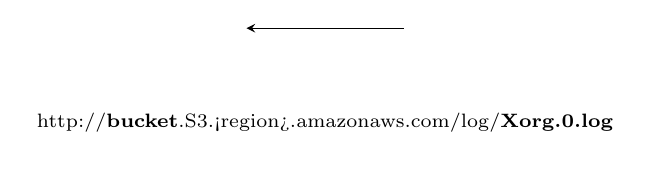
\begin{tikzpicture}[scale=1, transform shape]
		\node at (0,-1.5) {\scriptsize http://\textbf{bucket}.S3.<region>.amazonaws.com/log/\textbf{Xorg.0.log}};
		\bucket{-1.5}{0}{0.3}{\tiny bucket}
		\file{1.5}{-0.3}{0.3}{\tiny log/Xorg.0.log}
		\draw[stealth-] (-1,-0.3) -- (1,-0.3);
	\end{tikzpicture}
	\end{center}
	\caption{Endereço S3}
	\end{figure}
	\framebreak
	\begin{itemize}
		\item Storage classes
			\begin{itemize}
				\item S3 Standard
				\item S3 Intelligent - Tiering
				\item S3 Standard - IA
				\item S3 One zone - IA
				\item S3 Glacier Instant Retrieval
				\item S3 Glacier Flexible Retrieval
				\item S3 Glacier Deep Archive
			\end{itemize}
	\end{itemize}
\end{frame}

\begin{frame}
	\frametitle{S3 Features}
	\begin{itemize}
	\begin{small}
		\item \textbf{S3 Storage class analysis}: Descobrir padrões de acesso
		\item \textbf{S3 Lifecycle policy}: Quando os dados devem ser transferidos para outro tipo de storage class
		\item \textbf{S3 Cross-Region Replication (CRR)}: Replicar buckets entre diferentes regiões
		\item \textbf{S3 Same Regnio Replication}: Replicar buckets na mesma região
		\item \textbf{S3 Object Lock}: Não permite que o bucket seja apagado
		\item \textbf{S3 Inventory}: Lista de objetos e status da criptografia
		\item \textbf{S3 Batch operations}: Copiar objetos de buckets, colocar tags, modificar acesso, etc\dots
		\item \textbf{S3 Select}: Aumenta a performace da query e reduz os custos
	\end{small}
	\end{itemize}
\end{frame}

\begin{frame}
	\frametitle{S3 Access Management}
	\begin{itemize}
		\item Buckets são privados por padrão
		\begin{itemize}
			\item O dono do recurso da acesso para os outros 
		\end{itemize}
		\item Resource-based policies
			\begin{itemize}
				\item Bucket policies: escrito em Json e permite/bloqueia usuários em determinado bucket
				\item Access Control Lists (ACLs) usa xml e define quem tem permissão para usar o bucket
			\end{itemize}
		\item User policies (IAM)
	\end{itemize}
\end{frame}

\section{Cloud Watch}

\begin{frame}
	\frametitle{Cloud Watch}
	\begin{itemize}
		\item Permite:
			\begin{itemize}
				\item Monitorar recursos e aplicações em tempo real
				\item Coletar métricas dos recursos e aplicações
				\item Criar alarmes que verificam métricas. Podem:
					\begin{itemize}
						\item Mandar notificações
						\item Fazer mudanças automáticas nos recursos
					\end{itemize}
			\end{itemize}
	\end{itemize}
\end{frame}


\section{IAM}

\begin{frame}
	\frametitle{IAM}
	\begin{itemize}
		\item \href{https://docs.aws.amazon.com/wellarchitected/latest/security-pillar/identity-and-access-management.html}{Identity and Acess Management}
		\item Boas práticas:
			\begin{itemize}
				\item Habilitar MFA
				\item Criar um usuário padrão para cada pessoa do time e dar permissões (Não usar o \textbf{root})
				\item Usar grupos para atribuir permissões
				\item Aplicar uma política de senhas do IAM
			\end{itemize}
		\item OBS: É universal, funciona em todas as regiões
	\end{itemize}
\end{frame}

\subsection{Usuários}

\begin{frame}
	\frametitle{IAM - Users}
	\begin{itemize}
		\item \textbf{Programmatic access}
		\item Enables an access key ID and secret access key for the AWS API, CLI, SDK, and other development tools.
		\begin{itemize}
			\item Instalar o CLI para ter acesso ao AWS
			\item Dar acesso de um bucket para uma aplicação
		\end{itemize}
		\item \textit{AWS Management Console access}
		\item Enables a password that allows users to sign-in to the AWS Management Console.
		\begin{itemize}
			\item Precisa dar permissão para esse usuário
		\end{itemize}
	\end{itemize}
\end{frame}

\subsection{Tags}

\begin{frame}
	\frametitle{IAM - Tags}
	\begin{itemize}
		\item Servem para a gente identificar serviços
		\item É possível fazer um relatório de faturamento baseado em \textit{Tags}
		\item \textbf{OBS}: É possível ter até 50 tags por serviço
	\end{itemize}
\end{frame}

\subsection{Policies}

\begin{frame}
	\frametitle{IAM - Políticas Pt.1}
	\begin{itemize}
		\item É uma boa prática criar grupos com permissões para os usuários. E não colocar permissões diretamente no usuário
		\item Permissões mais específicas são mais fortes (Permissão de usuário prevalece contra permissão de grupo)
		\item \href{https://docs.aws.amazon.com/pt_br/IAM/latest/UserGuide/id_credentials_passwords_account-policy.html}{Políticas de senha}
			\begin{itemize}
				\item Exigir que o usuário use senhas fortes
				\item Expiração de senhas
				\item Impedir reutilização de senhas
				\item Etc\dots
			\end{itemize}
	\end{itemize}
\end{frame}

\begin{frame}
	\frametitle{IAM - Políticas Pt.2}
	\begin{itemize}
		\item Políticas de acesso
			\begin{itemize}
				\item As políticas podem ser definidas por um arquivo Json
				\item Pode ser usado políticas prontas ou criar políticas específicas
				\item Então as políticas podem ser atribuídas em usuários/grupos
			\end{itemize}
	\end{itemize}
\end{frame}

\subsection{Roles}

\begin{frame}
	\frametitle{Funções/Roles}
	\begin{itemize}
		\item Dar permissões para:
			\begin{itemize}
				\item Recursos
				\begin{itemize}
					\item Ex: Dar permissão para uma instância acessar um bucket
				\end{itemize}
				\item Outras contas AWS
				\item Federações do SAML 2.0
				\item Identidade web (Login Google, amazon, etc\dots)
			\end{itemize}
	\end{itemize}
\end{frame}

\subsection{Relatórios}

\begin{frame}
	\frametitle{Relatórios de acesso}
	\begin{itemize}
		\item Relatórios de credenciais
			\begin{itemize}
				\item Lista de todas as credenciais geradas
			\end{itemize}
		\item Access Analyzer: Gera um relatório de políticas pra a gente ver o que precisa ser modificado. é possível arquivar, resolver, etc\dots
	\end{itemize}
\end{frame}

\section{IAM Identify Center}

\begin{frame}
	\frametitle{IAM Identify Center}
	\begin{itemize}
		\item Expande as capacidades da AWS IAM
		\item Provê um lugar centralizado para administrar os usuários e seus acessos para contas AWS e aplicações cloud
			\begin{itemize}
				\item Workforce identities
				\item Application assignments for SAML applications
				\item Identity Center enabled applications
				\item Multi-account permissions
				\item AWS access portal
			\end{itemize}
	\end{itemize}
\end{frame}

\subsection{Workforce identities}

\begin{frame}
	\frametitle{IAM - Users}
	\begin{itemize}
		\item a
	\end{itemize}
\end{frame}


\section{Extra}

\subsection{Reduce costs (Coiled)}

\begin{frame}
	\frametitle{Usando Spot (com Coiled)}
	\begin{itemize}
		\item Spots podem salvar muito dinheiro \cite{Spot}, mas você precisa:
			\begin{itemize}
				\item Encontrar máquinas Spots o suficiente na sua região
				\item Lidar com seu desaparecimento
			\end{itemize}
	\end{itemize}
\end{frame}

\begin{frame}
	\frametitle{Escolher AZ e Região \cite{AWSCETips}}
	\begin{itemize}
		\item Verificar se na sua zona tem Spots o suficiente
			\begin{itemize}
				\item  Usar o Spot placement score para ver qual região ou az tem mais chance de suprir as necessidades do usuário
			\end{itemize}
		\item Deixar todos os Spots em uma zona só (Evitar custos de transferência de dados por zona)
	\end{itemize}
\end{frame}

\begin{frame}
	\frametitle{Fallback}
	\begin{itemize}
		\item Se os Spots não forem o suficiente é possível colocar instâncias \it{On-demand} para suprir as necessidades
			\begin{itemize}
				\item Spot: Vai alocar apenas Spots
				\item Spot-with-fallback: Vai alocar Spots e vai alocar on-demand caso seja necessário
				\item On-demand: Se quiser que tudo seja estável
			\end{itemize}
	\end{itemize}
\end{frame}

%\section{Teoria}

\subsection{Cloud X Virtualização}

\begin{frame}
	\frametitle{Virtualização}
	\begin{itemize}
		\item Criação de infraestruturas virtuais a partir de uma estrutura física
	\end{itemize}
\end{frame}

\begin{frame}
	\frametitle{Cloud}
	\begin{itemize}
		\item Conceito que reúne vários \textit{softwares} e utiliza de virtualização
		\item Possui algumas características específicas:
			\begin{itemize}
				\item Autoserviço sob demanda
				\item Amplo acesso a rede
				\item Pool de recursos
				\item Rápida elaticidade
				\item Serviços mensuráveis
			\end{itemize}
		\item \textbf{Colocation}: 1000 \textbf{VMs} na rede, \textbf{VPS} por um provedor, servidor físico em um provedor, etc\dots
	\end{itemize}
\end{frame}

\subsection{Cloud para o NIST}

\begin{frame}
	\frametitle{NIST}
	\begin{itemize}
		\item Um modelo para habilitar o acesso por rede a um conjunto compartilhado de recursos de computação e precisa ser:
			\begin{itemize}
				\item Ubíquo (Pode ser encontrado em todos os lugares)
				\item Conveniente
				\item Sob demanda
			\end{itemize}
		\item \textbf{Recursos de computação}: Redes, servidores, armazenamento, aplicações e serviços
		\item Esses recursos devem ser provisionados e liberados com o mínimo de esforço de gerenciamento ou interação com o provedor de serviços.
	\end{itemize}
\end{frame}

\begin{frame}
	\frametitle{Características}
	\begin{itemize}
		\item \textbf{Auto-serviço sob demanda}
		\item \textbf{Amplo acesso por rede}
		\item \textbf{Agrupamento de recursos}
		\item \textbf{Elasticidade rápida}
		\item \textbf{Serviço mensurado}
	\end{itemize}
\end{frame}

\begin{frame}
	\frametitle{Auto-serviço sob demanda}
	\begin{itemize}
		\item O consumidor pode providionar por conta própra \textbf{Recursos de computação}
		\item Não necessita da intervenção humana dos provedores de serviço
	\end{itemize}
\end{frame}

\begin{frame}
	\frametitle{Amplo acesso por rede}
	\begin{itemize}
		\item Os \textbf{Recursos de computação} estão disponíveis através da rede
		\item São acessados através de mecanismos padronizados que promovem o uso por dispositivos, clientes leves ou ricos de diversas plataformas (Smartphones, tablets, laptops ou desktops)
	\end{itemize}
\end{frame}

\begin{frame}
	\frametitle{Agrupamento de recursos}
	\begin{itemize}
		\item Os \textbf{Recusos de computação} do provedor são agrupados para atender a múltiplos consumidores em modalidade multi-inquilinos (Recursos físicos e virtuais diferentes dinamicamentes atribuídos e reatribuídos conforme a demanda dos consumidores)
		\item Há uma certa independência de localização geográfica, uma vez que o consumidor em geral não controla ou conhece a localização exata dos recursos fornecidos
		\item Mas pode ser capaz de especificar a localização em um nível de abstração mais alto (país, estado, datacenter)
	\end{itemize}
\end{frame}

\begin{frame}
	\frametitle{Elasticidade rápida}
	\begin{itemize}
		\item Os recursos podem ser provisionados e liberados elasticamente, em alguns casos automaticamentes, para rapidamente aumentar ou diminuir de acordo com a demanda
		\item Para o consumidor, os recursos disponíveis para provisionamento muitas vezes parecem ser ilimitados e podem ser alocados em qualquer quantidade e a qualquer tempo
	\end{itemize}
\end{frame}

\begin{frame}
	\frametitle{Serviços mensurado}
	\begin{itemize}
		\item Os sistemas na nuvem automaticamente controlam e otimizam o uso dos recursos através de medições em um nível de abstração apropriado para o tipo de serviço (como armazenamento, processamento, comunicação de ree e contas de usuário ativas)
		\item A utilização de recursos pode ser monitorada, controlada e informada, gerando transparência tanto para o fornecedor como para o consumidor do serviço utilizado
	\end{itemize}
\end{frame}

\subsection{Papéis e atividades no cloud}

\begin{frame}
	\frametitle{Papéis e atividades do profissional cloud}
	\begin{itemize}
		\item \textbf{Consumidor de nuvem}
		\item \textbf{Provedor de nuvem}
		\item \textbf{Broker de nuvem}
		\item \textbf{Auditor}
		\item \textbf{Operadora de nuvem}
	\end{itemize}
\end{frame}

\begin{frame}
	\frametitle{Consumidor de nuvem}
	\begin{itemize}
		\item Uma pessoa/organização que mantém relação comercial com o fornecedor da nuvem, e usa o serviço
		\item Uso:
			\begin{itemize}
				\item Um consumidor de nuvem procura o catálogo de serviços de um provedor de nuvem
				\item Solicita o serviço apropriado
				\item Configura contratos de serviço com o provedor da nuvem
				\item Usa o serviço
			\end{itemize}
		\item O consumidor pode ser cobrado pelo serviço fornecido e precisa organizar os pagamentos de acordo
		\item \textbf{OBS}: Dependendo dos serviços solicitados, as atividades e os cenários de uso podem ser diferentes entre os consumidores da nuvem
	\end{itemize}
\end{frame}

\begin{frame}
	\frametitle{Provedor de nuvem}
	\begin{itemize}
		\item Um provedor de nuvem pode ser uma pessoa, uma organização ou uma entidade responsável por disponibilizar um serviço aos consumidores de nuvem
		\item Um provedor de nuvem:
			\begin{itemize}
				\item Cria o software/plataforma/serviços de infraestrutura solicitados
				\item Gerencia a infraestrutura técnica necessária para fornecr os serviços
				\item Providencia os acordos de níveis de serviço (SLA) e protege a segurança e a privacidade dos serviços
			\end{itemize}
	\end{itemize}
\end{frame}

\begin{frame}
	\frametitle{Broker de nuvem}
	\begin{itemize}
		\item Uma entidade que
			\begin{itemize}
				\item Gerencia o uso
				\item Desempenho
				\item Entrega de serviços na nuvem
				\item Negocia relaões entre o \textbf{Provedor de nuvem} e o \textbf{Consumidor de nuvem}
			\end{itemize}
	\end{itemize}
\end{frame}

\begin{frame}
	\frametitle{Auditor}
	\begin{itemize}
		\item Pode avaliar os serviços fornecidos por um \textbf{Provedor de nuvem}:
			\begin{itemize}
				\item Controles de segurança
				\item Impacto de privacidade
				\item Desempenho
				\item Aderência aos parâmetros do acordo de nível de serviço (SLA)
			\end{itemize}
	\end{itemize}
\end{frame}

\begin{frame}
	\frametitle{Operadora de nuvem}
	\begin{itemize}
		\item Um intermediário que fornece conectividade e transporte de serviços na nuvem entre \textbf{Consumidores de nuvem} e \textbf{Provedores de nuvem}
		\item As operadoras de nuvem fornecem acesso aos consumidores através de redes, telecomunicações e outros dispositivos de acesso (computadores, laptops, telefones celulares, etc\dots)
		\item A distribuição de serviços na nuvem é normalmente fornecida por operadoras de rede e telecomunicações ou por um agente de transporte
	\end{itemize}
\end{frame}

\subsection{Tipos de nuvem}

\begin{frame}
	\frametitle{Tipos de nuvem}
	\begin{itemize}
		\item \textbf{Infraestrutura como Serviço (Iaas)}
		\item \textbf{Software como Serviço (SaaS)}
		\item \textbf{Plataforma como Serviço (PaaS)}
	\end{itemize}
\end{frame}

\begin{frame}
	\frametitle{IaaS - Infrastructure as a Service}
	\begin{itemize}
		\item O recurso fornecido ao consumidor é provisionar:
			\begin{itemize}
				\item Processamento
				\item Armazenamento
				\item Comunicação de rede
				\item Outros recursos de computação funcamentais nos quais o consumidor pode instalar e executar softwares em geral, incluindo sistemas operaionais e aplicativos
				\item Possivelmente um controle limitado de alguns componentes de rede (\textit{firewall})
			\end{itemize}
	\end{itemize}
\end{frame}

\begin{frame}
	\frametitle{PaaS - Plataform as a Service}
	\begin{itemize}
		\item O recurso fornecido ao consumidor é instalar na infraestrutura na nuvem aplicativos criados ou adiquiridos pelo consumidor,
		\item O consumidor tem controle sobre as aplicações instaladas e possívelmente configuraçoes de hospedagem de aplicações
		\item O consumidor não gerencia nem controla a infraestrutura na nuvem subjacente (Rede, servidores, sistemas operacionais, armazenamento ou mesmo recursos individuais da aplicação, com a possível exeção de configurações limitadas por usuário)
	\end{itemize}
\end{frame}

\begin{frame}
	\frametitle{SaaS - Software as a Service}
	\begin{itemize}
		\item O recurso fornecido ao consumidor é o uso de aplicções do fornecedor executando em uma infraestrutura na nuvem
		\item As aplicações podem ser acessadas por vários dispositivos clientes através de interfaces leves ou ricas
		\item O consumidor não gerencia nem controla a infraestrutura na nuvem subjacente (Rede, servidores, sistemas operacionais, armazenamento ou mesmo recursos individuais da aplicação, com a possível exeção de configurações limitadas por usuário)
	\end{itemize}
\end{frame}

\begin{frame}
	\frametitle{Exemplos}
	\begin{tiny}
	\begin{table}[ht]
		\centering
		\begin{tabular}{|p{1cm}|p{5cm}|p{4cm}|}
		\hline
			Tipo & Serviço & Exemplos \\
		\hline
		\hline
		  \multirow{3}{*}{IaaS}
			& Rede virtualizada & AWS VPC, Azura Virtual Network \\
			& Armazenamento de dados & AWS S3, Google cloud storage \\
			& Servidores Virtuais & AWS EC2, Azure Virtual Machines \\
			\hline
		  \multirow{2}{*}{PaaS}
			& Infraestrutura para desenvolvimento, implantação e execução de aplicativos & Heroku, Google App Engine \\
			& Plataforma testes e gerenciamento de aplicações & AWS Elastic Beanstalk \\
			\hline
		  \multirow{3}{*}{SaaS}
			& Armazenamento Dados & DropBox, Google Drive \\
			& Editor de textos e planilha & Gsuite e Office 365 \\
			& SIstema de Gestão de banco de dados & AWS RDS, Google Cloud SQL \\
		\hline
		\end{tabular}
		\caption{Exemplos de serviços}
	\end{table}
	\end{tiny}
\end{frame}

\subsection{Categorias de Serviços de nuvem}

\begin{frame}
	\frametitle{Categorias de Serviços de nuvem}
	\begin{itemize}
		\item \textbf{Comunicação como serviço (CaaS)}
		\item \textbf{Computação como serviço (CompaaS)}
		\item \textbf{Armazenamento de dados como serviço (DSaaS)}
		\item \textbf{Rede como serviço (NaaS)}
		\item \textbf{Banco de dados como serviço (DBaaS)}
	\end{itemize}
\end{frame}

\begin{frame}
	\frametitle{Comunicação como serviço (CaaS)}
	\begin{itemize}
		\item As capacidades oferecidas ao cliente do serviço de nuvem são a interação e a colaboração em tempo real
	\end{itemize}
\end{frame}

\begin{frame}
	\frametitle{Computação como serviço (CompaaS)}
	\begin{itemize}
		\item As capacidades oferecidas ao cliente do serviço de nuvem são a provisão e o uso de recursos de processamento necessários à implantação e execucão de softwares
	\end{itemize}
\end{frame}

\begin{frame}
	\frametitle{Armazenamento de dados como serviço (DSaaS)}
	\begin{itemize}
		\item As capacidades oferecidas ao cliente do serviço de nuvem são a provisão e o uso de armazenamento de dados e suas capacidades relacionadas
	\end{itemize}
\end{frame}

\begin{frame}
	\frametitle{Rede como serviço (NaaS)}
	\begin{itemize}
		\item As capacidades oferecidas ao cliente do serviço de nuvem são a conectividade para o transporte e as capacidades relacionadas à rede
	\end{itemize}
\end{frame}

\begin{frame}
	\frametitle{Banco de dados como serviço (DBaaS)}
	\begin{itemize}
		\item Oferece a funcionalidade d eum banco de dados semelhante ao que é encontrado em SGBDs
	\end{itemize}
\end{frame}

\subsection{Modelos de implementação de nuvem}

\begin{frame}
	\frametitle{Modelos de implementação de nuvem}
	\begin{itemize}
		\item Nuvem pública
		\item Nuvem privada
		\item Nuvem híbrida
		\item Nuvem comunitária
	\end{itemize}
\end{frame}

\begin{frame}
	\frametitle{Nuvem pública}
	\begin{itemize}
		\item Provisionada para uso aberto ao público em geral
		\item Sua propriedade, gerenciamento e operação podem ser de:
			\begin{itemize}
				\item Uma empresa
				\item Uma instituição acadêmica
				\item Uma organização do governo
				\item Ou uma combinação mista
			\end{itemize}
		\item Fica nas instalações do fornecedor
	\item \textbf{OBS}: Criar uma estrutura na Amazon e configurar usando VPN ou conexão direta continua sendo uma nuvem pública
	\end{itemize}
\end{frame}

\begin{frame}
	\frametitle{Nuvem privada}
	\begin{itemize}
		\item Provisionada para uso exclusivo por uma únic organização composta de diversos consumidores
		\item A sua propriedade, gerenciamento de operação podem ser de:
			\begin{itemize}
				\item A própria organização
				\item Terceiros
				\item Combinação mista
			\end{itemize}
		\item Pode estar dentro ou fora das instalações da organização
		\item Nuvem privada não é organização e não precisa estar instalada localmente
	\end{itemize}
\end{frame}

\begin{frame}
	\frametitle{Nuvem comunitária}
	\begin{itemize}
		\item Provisionada para uso exclusivo por uma determinada comunidade de consumidores de organizações que têm interesses em comum (missão, requisitos de segurança, políticas, observância de regulamentações)
		\item A sua propriedade, gerenciamento e operação podem ser de:
			\begin{itemize}
				\item Uma organização
				\item Mais de uma organizações da comunidade
				\item Terceiros
				\item Combinação mista
			\end{itemize}
		\item Pode estar dentro ou fora das instalações das organizações participantes
	\end{itemize}
\end{frame}

\begin{frame}
	\frametitle{Nuvem híbrida}
	\begin{itemize}
		\item Composição de duas ou mais infraestruturas na nuvem (\textbf{privadas}, \textbf{comunitárias} ou \textbf{públicas}) que permanecem entidades distintas
		\item São interligadas por tecnoogia padronizada ou proprietária que permite a comunicação de dados e portabilidade de aplicações (Transferencia de processamento para a nuvem para balanceamento de carga entre nuvens)
	\end{itemize}
\end{frame}

\subsection{Arquitetura de Aplicações}

\begin{frame}
	\frametitle{Single-tenant X Multi-tetant}
	\begin{multicols}{2}
		\begin{itemize}
			\item \textbf{Single-tenant}
			\item \tiny Várias empresas compartilham a mesma instância para armazenamento
			\item \tiny Instância é dividida/particionada para que as empresas não acessem informações de outra
			\item \tiny Benefícios
				\begin{itemize}
					\item \tiny Máxima privacidade: 1 instância por usuário
					\item \tiny Sem prioridades
					\item \tiny Pode usar os recursos como quiser
				\end{itemize}
			\item \tiny Desvantagens
				\begin{itemize}
					\item \tiny Custear todo sistema sozinho
					\item \tiny O uso do sistema não é o mais eficiente
				\end{itemize}
		\end{itemize}
		\columnbreak
		\begin{itemize}
			\item \textbf{Multi-tenant}
			\item \tiny Cada empresa possui sua própria instância do aplicativo e infra-estrutura
			\item \tiny Benefícios
				\begin{itemize}
					\item \tiny Economia de Hardware e energia (custo)
					\item \tiny Esforço maior para atualizar
					\item \tiny Backup e Redundância mais fáceis em relação ao Single-tenant
				\end{itemize}
			\item \tiny Desvantagens
				\begin{itemize}
					\item \tiny Menos customização específica
					\item \tiny Menos autorização e Atraso de tempo (Recursos ou funcionalidades podem ser adiadas, empresas maiores ganham preferencia)
				\end{itemize}
		\end{itemize}
		
	\end{multicols}
\end{frame}

\begin{frame}
	\frametitle{Inquilino isolado}
	\begin{itemize}
		\item Cada inquilito tem seu próprio stack de tecnologia, não havendo compartilhamento de recursos
		\item Para uma oferta SaaS, este modelo carece de agilidade e de elasticidade, porque adicionar um novo inquilino requer o provisionamento de sua própria instância de hardware e de software
		\item Embora não seja verdadeiramente Computação em Nuvem, é um passo nessa direção, oferecendo como atrativo a facilidade de uma rápida oferta para SaaS
	\end{itemize}
\end{frame}

\begin{frame}
	\frametitle{Multi-inquilino (Virtualização)}
	\begin{itemize}
		\item Cada inquilino tem seu próprio stack de tecnologia, mas o hardware é alocado dinamicamente a partir de um pool de recursos, via mecanismos de virtualização
		\item Bastante similar ao modelo anterior, mas permitindo elasticidade na camada do hardware
		\item Entretanto, apresenta limitações, pois a unidade de alocação e liberação de recursos é a máquina virtual onde aplicação vai operar.
	\end{itemize}
\end{frame}

\begin{frame}
	\frametitle{Multi-inquilino via container}
	\begin{itemize}
		\item Vários inquilinos são executados na mesma instância de um container de aplicação (um servidor de aplicações), mas cada inquilino está associado a uma instância separada do software de banco de dados
		\item O ambiente de execução é compartilhado entre vários inquilinos, mas a plataforma de dados é a mesma
		\item Premissa do modelo é que o isolamento do banco de dados garante integridade dos dados dos inquilinos, ao mesmo tempo em que o container de execução, por ser compartilhado, oferece as vantagens de elasticidade e de customização
	\end{itemize}
\end{frame}

\begin{frame}
	\frametitle{Multi-inquilino via todo o stack de software compartilhado}
	\begin{itemize}
		\item É uma evolução do modelo anterior, agora com todo o stack de software sendo compartilhado
		\item Neste modelo, além do container da aplicação, também uma única instância do banco de dados é compartilhada por todos os inquilinos
		\item \href{https://www.youtube.com/watch?v=S9_K1jwjo1U}{Vídeo explicativo}
	\end{itemize}
\end{frame}

\subsection{Pontos para considerar migração}

\begin{frame}
	\frametitle{Devo migrar?}
	\begin{itemize}
		\item \textbf{Custo real}: Verificar se o modelo atual usado pela empresa tem um custo mais alto do que o modelo de computação em nuvem
		\item \textbf{Confiabilidade}: É muito importante avaliar a reputação do provedor de nuvem, e também as políticas de segurança desse provedor
		\item \textbf{Legalidade}: Nem todas as empresas podem mover suas aplicações para nuvens públicas, e um dos motivos são os fatores legais, regulamentações do tipo de negócio ou país que a empresa opera, que não permitem que os dados estejam localizados fora do país.
	\end{itemize}
\end{frame}

\begin{frame}
	\frametitle{Custo real}
	\begin{itemize}
		\item Deve ser levado em conta:
		\begin{itemize}
			\item Quanto de armazenamento será necessário
			\item Qual o poder computacional vai precisar como processamento e outros
			\item Quanto de tráfego vai utilizar
			\item O valor de licença de software
			\item Contratar pessas para desenvolver aplicações para nuvem? Capacitar a equipe?
			\item Investir dinheiro em certificações e para se adaptar às regulamentações da empresa
			\item Custos inesperados como customização de aplicações
			\item Transferência de dados
			\item Custos de validação
			\item Outros
		\end{itemize}
		\item Após somar tudo isso certifique que o ROI (retorno sobre o investimento) seja favorável para a migração.
	\end{itemize}
\end{frame}

\subsection{Modelo de nuvem ideal}

\begin{frame}
	\frametitle{Custo real}
	\begin{tiny}
	\begin{itemize}
		\item Se você quer reduzir custos operacionais de atualização, manutenção e licenciamento de software ou se você tem uma empresa pequena ou de médio porte mas não tem pessoal suficiente para manter a TI mas precisa de tecnologia de ponta, ou se a empresa não dispõe de recursos para investir em infraestrutura e precisa de tecnologia de ponta o modelo ideal é a nuvem pública
		\item Mas se a empresa quer ter o controle de todo o datacenter, servidores, softwares, segurança ou por questões legais não pode hospedar seus serviços fora da empresa aí você deve utilizar nuvem privada
		\item Mas tem um outro caso que é a empresa que gosta de manter o controle dos dados locais mas também gostaria de oferecer alguns serviços que estão disponíveis em nuvem pública, neste caso você utiliza uma estrutura com nuvem híbrida, e isso é o que vem acontecendo com a maioria das empresas
	\end{itemize}
	\end{tiny}
\end{frame}

\subsection{Escolher um provedor}

\begin{frame}
	\frametitle{Custo real}
	\begin{tiny}
	\begin{itemize}
		\item Responsabilidade do provedor: Você precisa ler o contrato que o provedor disponibiliza
		\item Recuperação contra desastre: Saber se o provedor tem um plano de contingência em caso de falha do serviço principal, isso vale mais para SaaS.
		\item Modelo de adoção suportados pelo provedor: Verificar, e se o provedor suporta a integração da nuvem pública com a sua nuvem privada para poder criar uma nuvem híbrida.
		\item Segurança dos dados: O que é responsabilidade do provedor e o que é sua responsabilidade, na maioria das vezes a segurança é compartilhado, o provedor disponibiliza as ferramentas, mas você precisa utilizá-las, conhecer as certificações que o provedor tem na área de segurança também é muito importante.
		\item Modelo de controle de identidade: pesquisar os tipos de controle de acesso fornecidos pela nuvem, saber se é possível fazer a integração de seus usuário locais com os usuários na nuvem, utilizando o mesmo modelo de autenticação.
		\item Manutenção dos serviços: Saber como são os procedimentos de manutenção, e isso serve para qualquer modelo de nuvem.
		\item Visão futura: É muito importante você saber quais são os projetos do provedor para o futuro, saber se tem algo que eles não ofereçam hoje mas vão oferecer no futuro, pois essa é uma parceria de longo prazo, não pense só no presente.
		\item Desempenho: Muitos provedores disponibilizam um período para você fazer testes e validar se o desempenho satisfaz as suas necessidades.
		\item Flexibilidade: Você deve saber se o seu provedor tem flexibilidade de customização, isso é muito importante principalmente para o modelo SaaS e também flexibilidade nos termos contratuais, isso pode tornar a negociação menos complicada.
		\item Segurança física: É muito importante procurar documentações e conhecer as certificações que provem a segurança física dos datacenters dos provedores.
	\end{itemize}
	\end{tiny}
\end{frame}

\begin{frame}
	\frametitle{Service Level Agreement (SLA)}
	\begin{itemize}
		\item Alguns exemplos de SLA da AWS e da Microsoft.
		\begin{itemize}
			\item \url{https://aws.amazon.com/pt/rds/sla/}
			\item \url{https://aws.amazon.com/pt/ec2/sla/}
			\item \url{https://aws.amazon.com/pt/s3/sla/}
			\item \url{https://azure.microsoft.com/pt-br/support/legal/sla/virtual-machines/v1_6/}
			\item \url{https://azure.microsoft.com/pt-br/support/legal/sla/storage/v1_2/}
			\item \url{https://contaazul.com/termos/}
	\end{itemize}
	\end{itemize}
\end{frame}



\begin{frame}[allowframebreaks]
\frametitle{Referencias}
\printbibliography
\end{frame}

\end{document}
